% Author-composition scaffold. This is intentionally not a completed submission.
\documentclass[10pt,letterpaper]{article}
\usepackage{spconf}
\usepackage[T1]{fontenc}
\usepackage{amsmath,amssymb,graphicx,booktabs,url}
\usepackage[hidelinks]{hyperref}
\title{ReCheck: Auditing Full-Progress Scores Against Executed Effects in LLM Agents}
% This file must be filled by the real author; the research is not anonymous.
\name{Author names pending}
\address{Department, institution, city, country pending \\
Contact email pending \\
{\fontsize{9}{10.8}\selectfont AI-generated research working draft; not for direct submission}}

\begin{document}
\maketitle
\begin{abstract}
\textbf{AUTHOR TEXT REQUIRED.} Compose approximately 100--150 words from the verified study, distinguishing saved model records, scripted controls, and local effect checks.
\end{abstract}
\begin{keywords}
Agent evaluation, tool use, benchmark auditing, temporal reasoning, outcome verification
\end{keywords}
\section{Introduction}
\textbf{AUTHOR TEXT REQUIRED.} State the research question and the narrow empirical contribution. Do not claim a new planning method or verified leaderboard change.
\section{Related Work}
\textbf{AUTHOR TEXT REQUIRED.} Compare ToolSandbox~\cite{toolsandbox}, TED~\cite{ted}, judge validation~\cite{judge}, tool-evaluator auditing~\cite{validity}, automated audits~\cite{aba}, and temporal reasoning~\cite{timebench}.
\section{Protocol and Data}
\textbf{AUTHOR TEXT REQUIRED.} Describe evidence identifiers, observed snapshot boundaries, active-request adjudication, calendar checks, abstention, data version~\cite{sapdata}, retrospective selection, and dependence between repeated templates.
\section{Results}
\textbf{AUTHOR TEXT REQUIRED.} Explain each denominator; retain ambiguous exclusions and the separate negative coverage.
\begin{table}[t]
\centering
\caption{Public effect-audit coverage. Full denotes source final progress equal to one; candidates precede contextual exclusions. Each template has 96 repeated records.}
\label{tab:tasks}
{\fontsize{9}{10.8}\selectfont
\setlength{\tabcolsep}{3pt}
\begin{tabular}{@{}lrrrr@{}}
\toprule
Task template & $N$ & Full & Cand. & Retained\\
\midrule
Reminder: specified date &96&68&5&1\\
Reminder: tomorrow &96&80&29&26\\
Reminder: next Friday &96&64&38&37\\
Contact from latest message &96&13&0&0\\
Message to a person &96&81&0&0\\
Message to a number &96&43&0&0\\
\midrule
Total &576&349&72&64\\
\bottomrule
\end{tabular}}
\end{table}

\begin{figure}[t]
\centering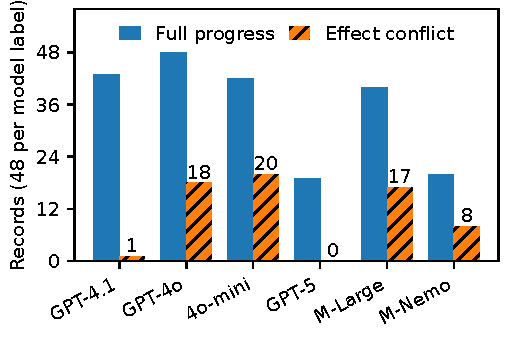
\includegraphics[width=\columnwidth]{figures/model_counts.pdf}
\caption{AUTHOR CAPTION REQUIRED. Six source labels; 48 reminder records each. The right-hand bars show retained score/effect conflicts, not re-ranked models.}
\end{figure}
\section{Temporal Controls}
\textbf{AUTHOR TEXT REQUIRED.} Explain why historical attainment and latest-state checks fail on different controls. These are scripted, not model-generated counterexamples.
\begin{table}[t]
\centering
\caption{One public two-stage task: change initial friends to enemies, then back to friends. Scripted controls, not model samples. End checks only the latest friend state; scoped checks both required stages.}
\label{tab:scope}
{\fontsize{9}{10.8}\selectfont
\setlength{\tabcolsep}{3.5pt}
\begin{tabular}{@{}lccc@{}}
\toprule
Trajectory & Source & End & Scoped\\
\midrule
Both stages completed &1.0&Yes&Yes\\
Second update omitted &0.8&No&No\\
Latest effect reversed &1.0&No&No\\
No write; completion claims &0.6&Yes&No\\
No-op error, then both stages &1.0&Yes&Yes\\
\bottomrule
\end{tabular}}
\end{table}

\section{Limitations and Conclusion}
\textbf{AUTHOR TEXT REQUIRED.} Bound the claim by observable effects and the fixed task subset. No causal diagnosis of the original judge and no general human-verified accuracy estimate were measured.
\begin{thebibliography}{7}
\bibitem{toolsandbox}
J. Lu, T. Holleis, Y. Zhang, B. Aumayer, F. Nan, H. Bai, S. Ma, S. Ma, M. Li, G. Yin, Z. Wang, and R. Pang,
``ToolSandbox: A stateful, conversational, interactive evaluation benchmark for LLM tool use capabilities,''
in \emph{Findings of NAACL}, 2025, pp. 1160--1183, doi: 10.18653/v1/2025.findings-naacl.65.
\bibitem{ted}
P. Chong, H. Abichandani, J. Shen, A. Ghosh, M. P. Moe, Y. Mai, and D. Dahlmeier,
``Talk, Evaluate, Diagnose: User-aware agent evaluation with automated error analysis,''
in \emph{ICLR}, 2026. Also arXiv:2603.15483v1.
\bibitem{judge}
L. Zheng et al., ``Judging LLM-as-a-Judge with MT-Bench and Chatbot Arena,''
in \emph{Advances in Neural Information Processing Systems}, vol. 36, 2023. Also arXiv:2306.05685.
\bibitem{validity}
J. Vaghasiya, V. Bhat, M. A. Mohsin, and A. Aali,
``Benchmarking the benchmarks: A validity audit of tool-calling evaluation,''
\emph{arXiv preprint arXiv:2607.02577v1}, 2026.
\bibitem{aba}
J. Wang, F. Bianchi, S. Zhu, F. Nie, Y. Kwon, B. Dhingra, and J. Zou,
``Automated benchmark auditing for AI agents and large language models,''
\emph{arXiv preprint arXiv:2605.26079v2}, 2026.
\bibitem{timebench}
Z. Chu, J. Chen, Q. Chen, W. Yu, H. Wang, M. Liu, and B. Qin,
``TimeBench: A comprehensive evaluation of temporal reasoning abilities in large language models,''
in \emph{Proc. ACL}, 2024, pp. 1204--1228, doi: 10.18653/v1/2024.acl-long.66.
\bibitem{sapdata}
SAP, ``Agent Quality Inspect: Public experiment records,'' Hugging Face dataset, 2026,
revision \texttt{593e686} (full commit in the artifact manifest).
\url{https://huggingface.co/datasets/SAP/agent-quality-inspect}.
\end{thebibliography}

\end{document}
